\chapter{Main part}
\label{sec:story}

% I'd like you to think about the work you have been doing on the alignment and what things have been investigated and what conclusions you have made. You want to build the story one piece at a time, so I think it will start with testing some of the constraints from the null tests and going from there. With the type of work you have been doing, you will also have a much larger "future work" and "continuing work" section, I would put it before the conclusion. This will be discussing things like the way we discovered the cluster bias and the way that it is linked to the rotational degrees of freedom, etc. And it can outline the things you know about the way the real detector will be aligned starting very soon.
% \begin{itemize}
%   \item testing some of the constraints from the null tests
%   \item future work: discovered cluster bias + link to rotational degrees of freedom
% \end{itemize}

% taking notes for now so i know what plots to use
% \begin{enumerate}
%   \item started with null tests.
%   \item which constraint does what?
%   \item which degree of freedom moves what part of the scifi?
% \end{enumerate}
\section{general info}

Alignment using tracks and vertices regarding stations layers and modules. testing constraints for different degrees of freedom with the goal to find the "perfect" configuration of constraints and alignable degrees of freedom.
Used the pre-installed alignment conditions with the survey constraints being
"FT : 0 0 0 0 0 0 : 1 1 1 0.0003 0.0003 0.0003”\\
"FT/T. : 0 0 0 0 0 0 : 1 1 1 0.0003 0.0003 0.0003”\\
"FT/T./Layer(X1|U|V|X2) : 0 0 0 0 0 0 : 0.2 0.2 0.2 0.0001 0.0001 0.0001”\\
"FT/.*Module. : 0 0 0 0 0 0 : 0.1 0.1 0.1 0.001 0.001 0.001"\\
"FT/.*Mat. : 0 0 0 0 0 0 : 0.05 0.05 0.05 0.1 0.1 0.1”\,.

The string is the name of the element, the first set of six numbers are hardcoded parameters for each of the 3 translation degrees of freedom and 3 rotational degrees of freedom (Tx, Ty, Tz, Rx, Ry, Rz) and the second set of six parameters are the corresponding uncertainties.
The scale for the translations are $\si{\milli\metre}$ and the scale for the rotations being $\si{\radiant}$. A survey uncertainty of $\num{0.0001}$ stands for $\SI{0.1}{\milli\radiant}$.

The alignments have been performed with gaudisplititer.

During the Alignment, lagrange constraints can be utilized to minimize the
$\chi^2$ under the condition
\begin{equation}
  f(\alpha) = 0
\end{equation}
and adding the lagrange parameter $\Lambda$ to get
\begin{equation}
  \Delta \chi^2 = \Lambda f(\alpha)
\end{equation}\,.

Lagrange constraints are added to fix losely constrained degrees of freedom and can be used for any linear combination of movements.

include table from https://twiki.cern.ch/twiki/bin/view/LHCb/TAlignmentManual.

\section{Nulltests and software tests}

As a starting point, Alignment v17r1 was used for 5000 events with the magnet in upward position and \textit{GoodLongTracks} (was sind goodlong tracks? definition von cuts etc.)

Results: (sort under the right plots) \\
\begin{itemize}
  \item Alignment with Rz (and Rx) takes lots of iterations to converge
  \item increasing nEvents does not improve it \to weak mode?
\end{itemize}

% compare 1000 to 7000 events for Tx flo versus my constraints.
% what exactly were flo's changes?
\begin{figure}
  \centering
  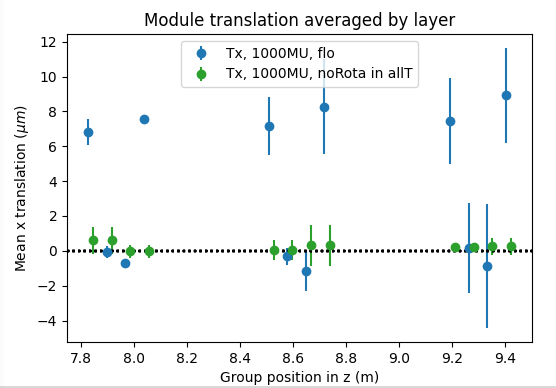
\includegraphics[width=0.8\textwidth]{plots/june_21/Tx_noRota_allT_1000MU.png}
  \caption{comparison of different configurations without rotational constraints in every station, magnet up and 1000 events. plotted is translation in x versus global z.}
  \label{fig:june_2}
\end{figure}

\begin{figure}
  \centering
  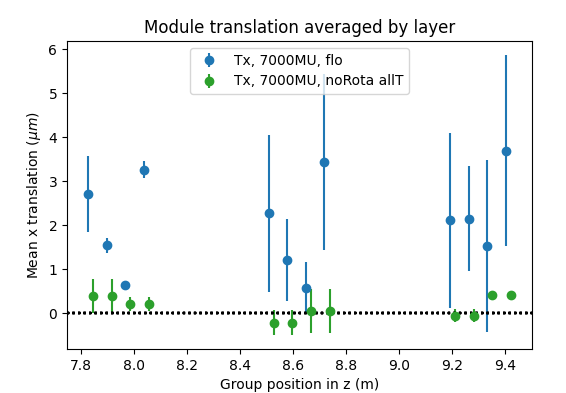
\includegraphics[width=0.8\textwidth]{plots/june_21/Tx_noRota_allT_7000MU.png}
  \caption{comparison of different configurations without rotational constraints in all stations, magnet up and 7000 events. plotted is x translation versus global z.}
  \label{fig:june_2}
\end{figure}

maybe show this plot \ref{fig:june_3}
\begin{figure}
  \centering
  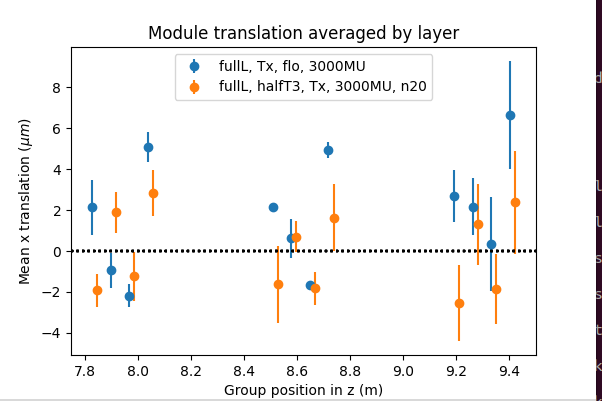
\includegraphics[width=0.8\textwidth]{plots/june_21/allT_halfT3_n20_Tx.png}
  \caption{analysed 20 iterations for x translation behavior (look up exact constraints and dofs)}
  \label{fig:june_3}
\end{figure}

\begin{figure}
  \centering
  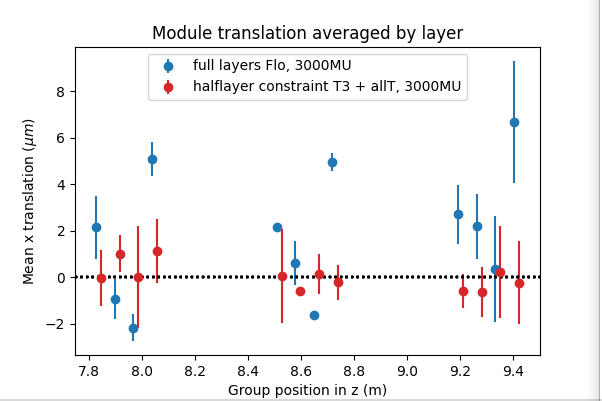
\includegraphics[width=0.8\textwidth]{plots/june_21/allT_halfT3_Tx_vs_Flo.png}
  \caption{halflayer constraints and full layer constraint, very strict (look up exact constraints and dofs)}
  \label{fig:june_4}
\end{figure}

the figure in \ref{fig:june_4} shows that very strict Tx constraints make Tx look better but when comparing to Tz as we can see in figure \ref{fig:june_5}
\begin{figure}
  \centering
  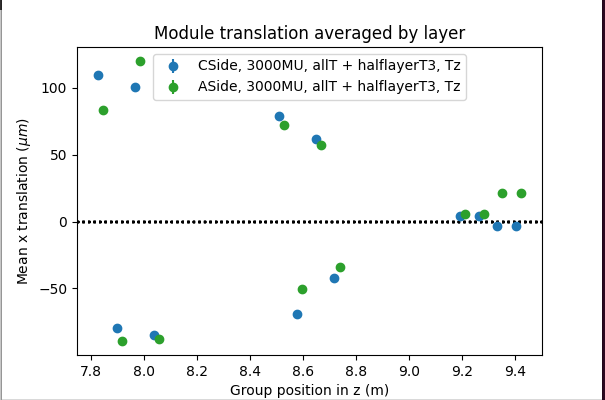
\includegraphics[width=0.8\textwidth]{plots/june_21/CA_allT_halfT3_Tz.png}
  \caption{compare C-Side to A-Side for Translation in z direction. (look up exact constraints and dofs)}
  \label{fig:june_5}
\end{figure}
a clear layer separation is visible. because of the many constraints that are applied to T3, a compensation is happening in the other two stations.

\begin{figure}
  \centering
  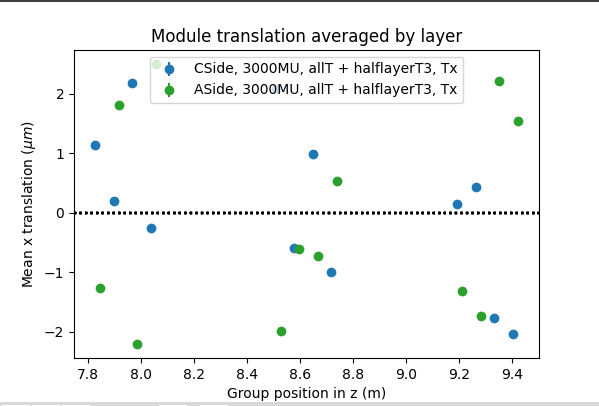
\includegraphics[width=0.8\textwidth]{plots/june_21/CA_allT_halfT3_Tx.png}
  \caption{compare C-Side to A-Side for Translation in x direction. (look up exact constraints and dofs)}
  \label{fig:june_6}
\end{figure}

Looking at figure \ref{fig:june_6}, the last two layers in station 3 are seperation from the first two. Especially the last station should be fixed around zero with the constraints added. The sum of all translations should be zero with each individual layer movement being small.

%\subsection{july plots}

test 3:
\begin{figure}
  \centering
  \begin{subfigure}[b]{0.3\textwidth}
    \centering
    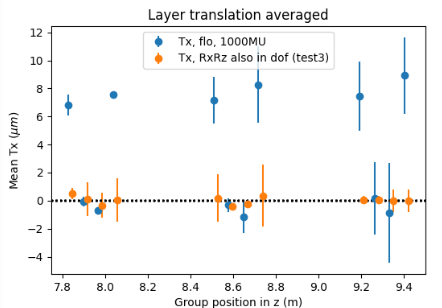
\includegraphics[width=\textwidth]{plots/july_28/Tx.png}
    \caption{Tx versus global z.}
  \end{subfigure}
  \hfill
  \begin{subfigure}[b]{0.3\textwidth}
    \centering
    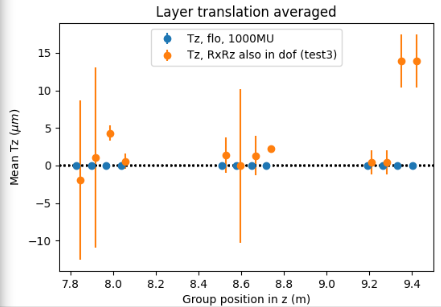
\includegraphics[width=\textwidth]{plots/july_28/Tz.png}
    \caption{Tz versus global z.}
  \end{subfigure}
  \hfill
  \begin{subfigure}[b]{0.3\textwidth}
    \centering
    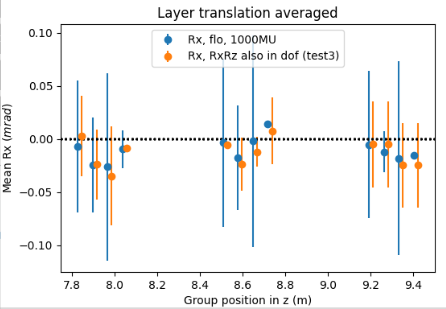
\includegraphics[width=\textwidth]{plots/july_28/Rx.png}
    \caption{Rx versus global z.}
  \end{subfigure}
  \caption{Testing a configuration versus florians changes.}
\end{figure}

%\subsection{august plots}
\begin{figure}
  \centering
  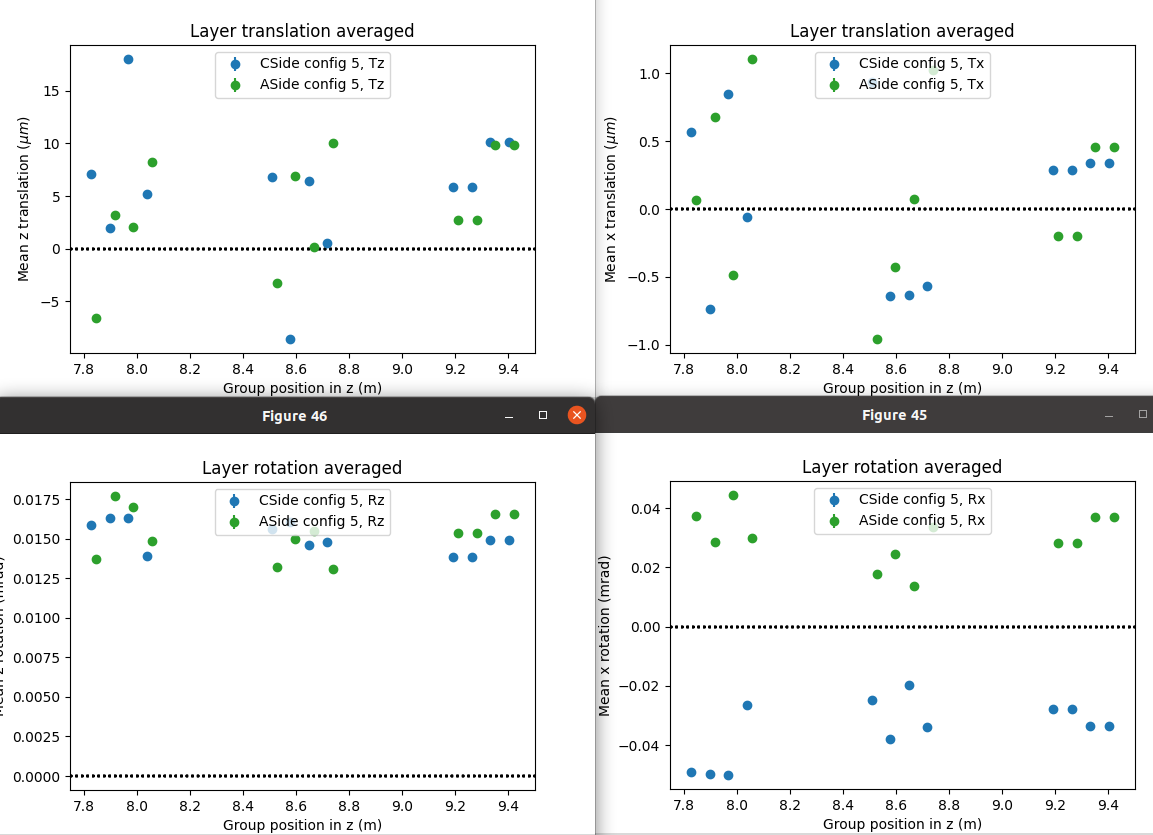
\includegraphics[width=0.8\textwidth]{plots/august_13/C_ASide_config5.png}
  \caption{old config 5, plotted C and ASide.}
  \label{fig:aug13_CA_old}
\end{figure}

\begin{figure}
  \centering
  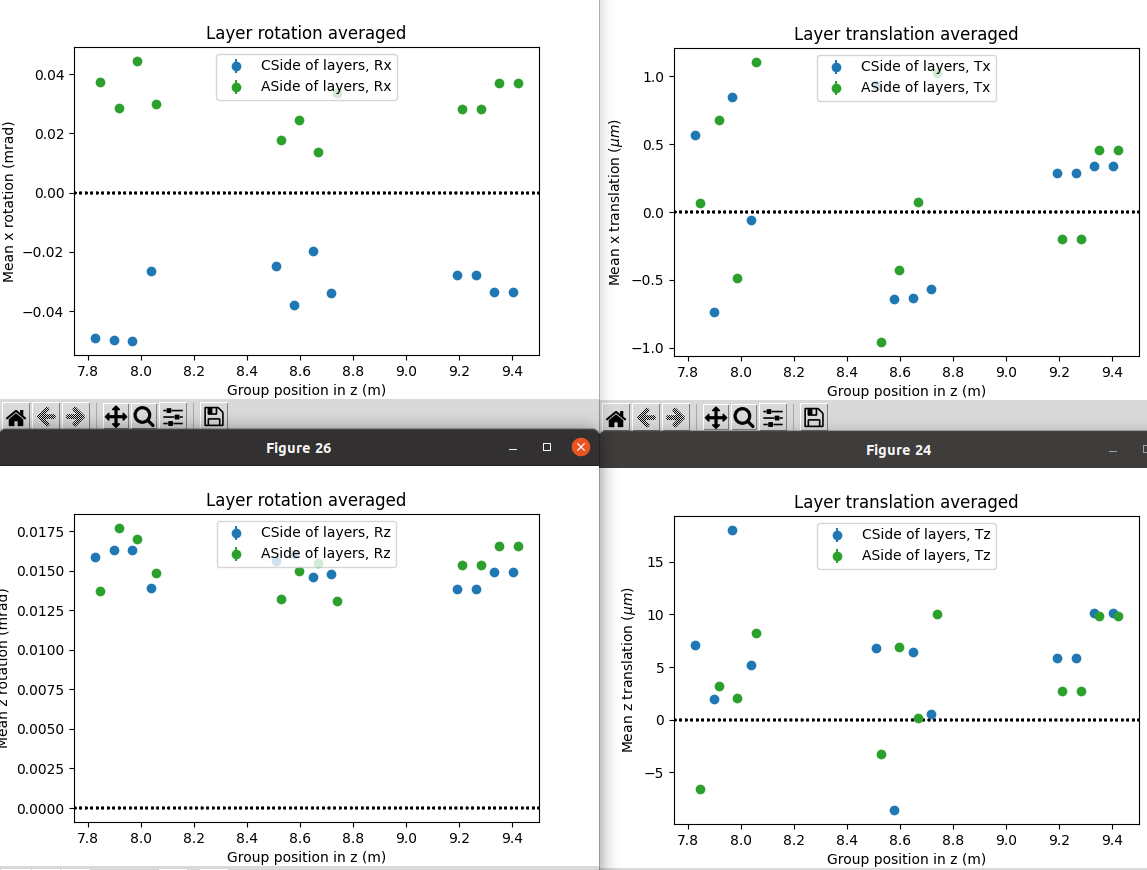
\includegraphics[width=0.8\textwidth]{plots/august_13/CA_side_newconfig5.png}
  \caption{new config 5, plotted C and ASide.}
  \label{fig:aug13_CA_new}
\end{figure}

\begin{figure}
  \centering
  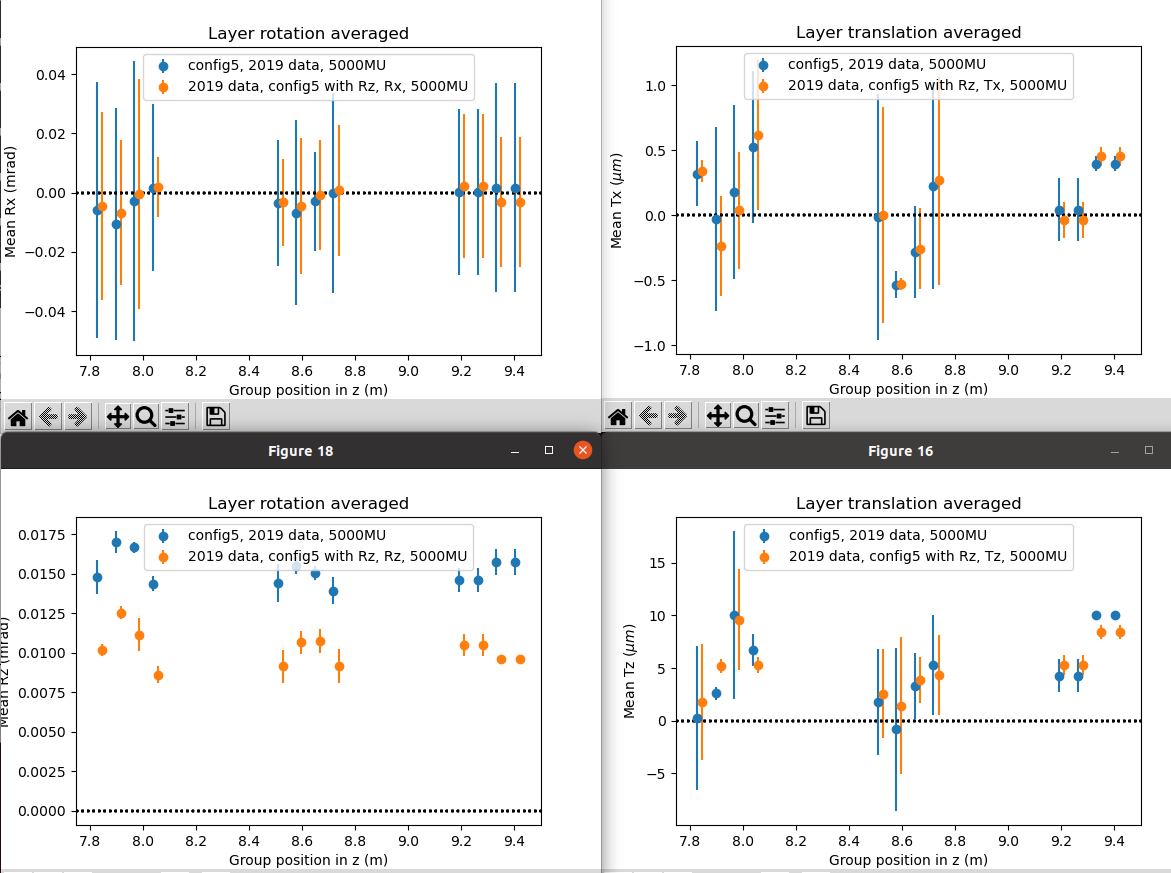
\includegraphics[width=0.8\textwidth]{plots/august_13/2019_c5_old_vs_withRz_MU.png}
  \caption{config5 versus config 5 with Rz constraint for rotational improvement.}
  \label{fig:withRz}
\end{figure}

\begin{figure}
  \centering
  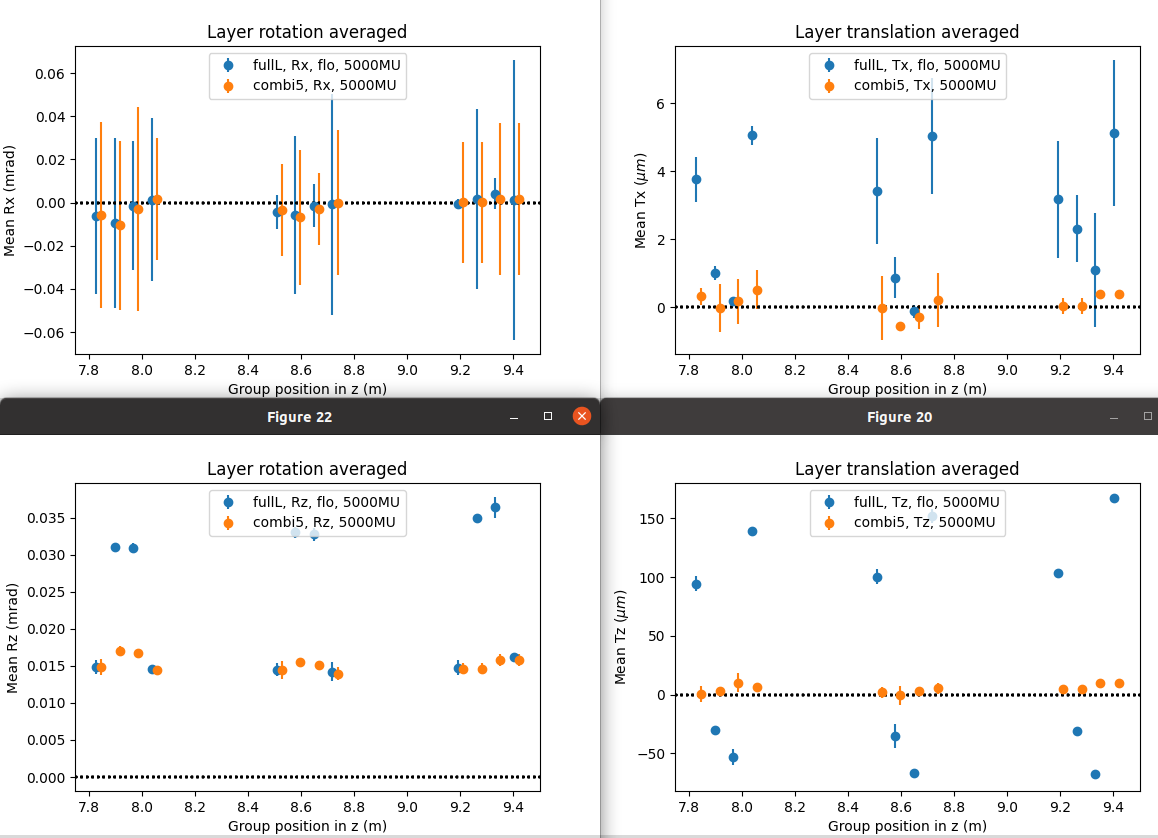
\includegraphics[width=0.8\textwidth]{plots/august_13/combi5_layers_averaged.png}
  \caption{flo with full layer constraint versus config 5}
  \label{fig:floFullL_c5}
\end{figure}

\begin{figure}
  \centering
  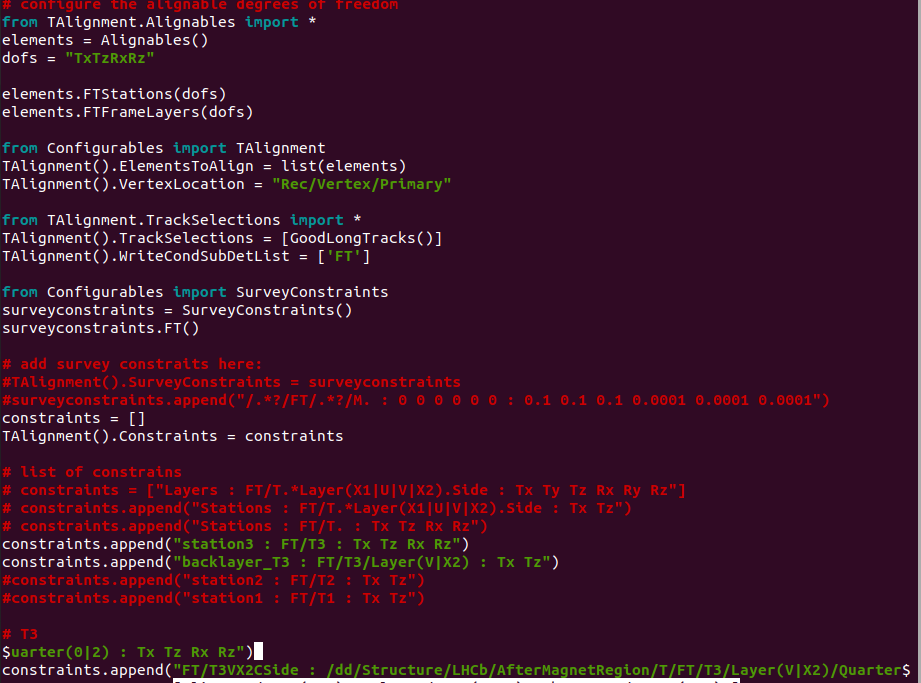
\includegraphics[width=0.8\textwidth]{plots/august_13/new_combi5_config.png}
  \caption{constraints for combi 5 used.}
  \label{fig:constraints_c5}
\end{figure}

\begin{figure}
  \centering
  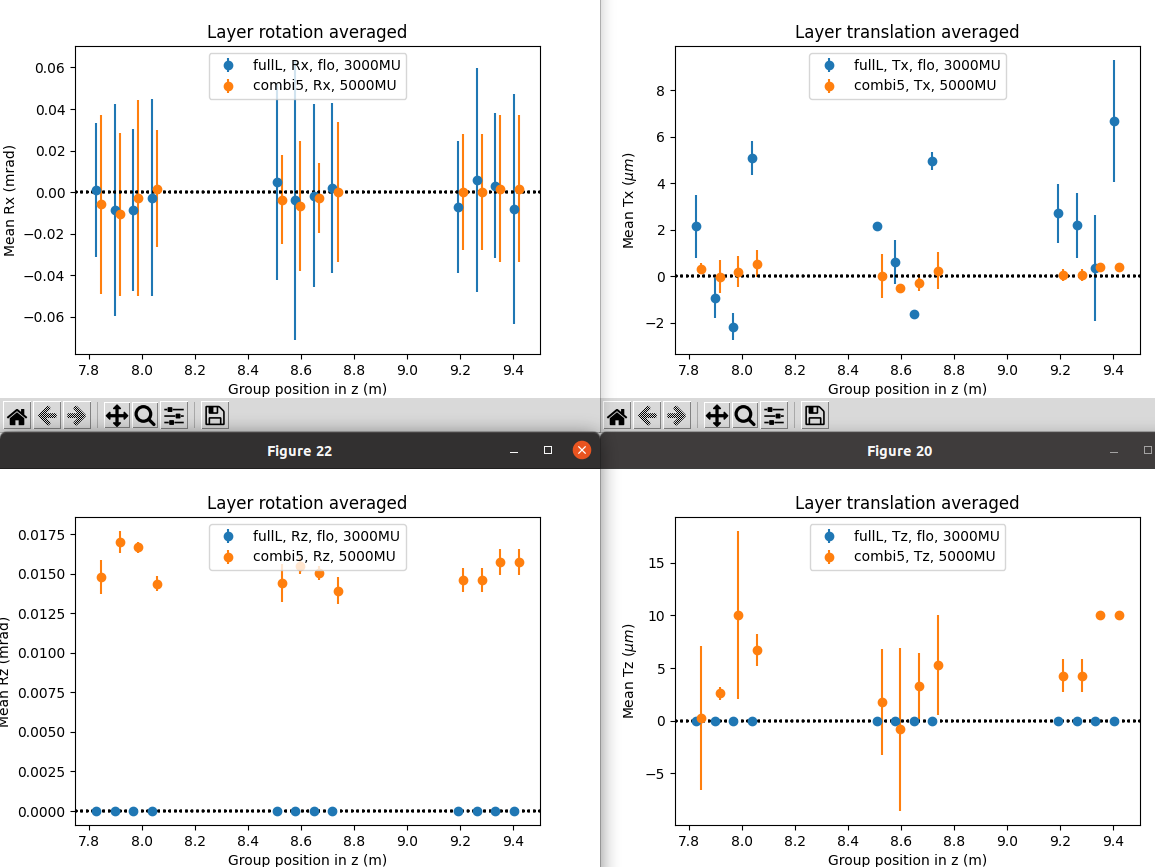
\includegraphics[width=0.8\textwidth]{plots/august_13/newCombi5.png}
  \caption{original new config 5, should be the first good plot to show!!}
  \label{fig:OGconfig5}
\end{figure}

% october plots
update: constraining backlayer and also aligning it (append dofs by : Rx Rz)
Results: \\
\begin{itemize}
  \item improves null tests for Rz but not the only reason why its shifted (cluster bias! expand later)
  \item shearing and scaling constraints do NOT improve this
\end{itemize}

Results of 100mu translation misalignment: \\
100mu translation misalignment matches expected survey uncertainty. BUT layers shifted from 0 !
TODO: FTTrackmonitor to study later splitting in track output

\begin{figure}
  \centering
  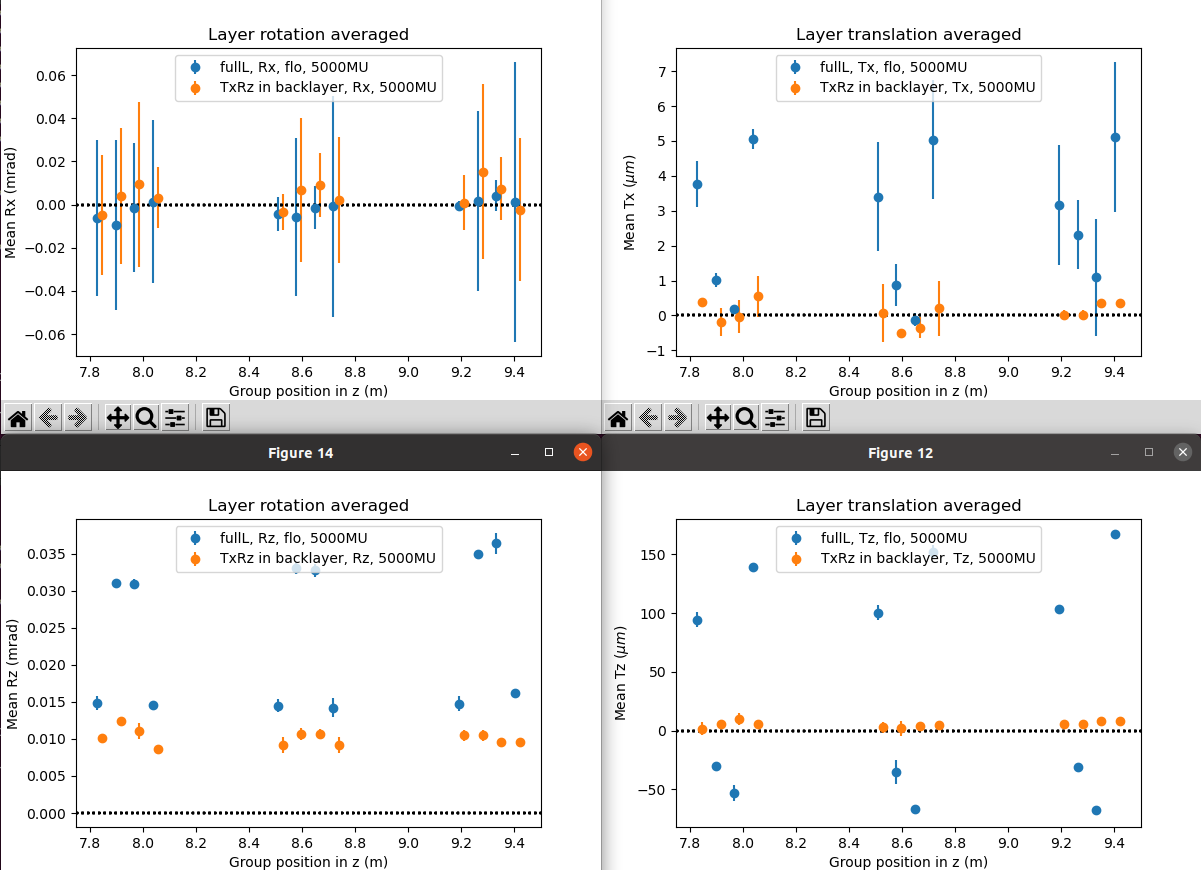
\includegraphics[width=0.8\textwidth]{plots/oct_4/TxRz_config5_backlayer.png}
  \caption{dofs Tx Rz and backlayer constraints.}
  \label{fig:oct4}
\end{figure}

\begin{figure}
  \centering
  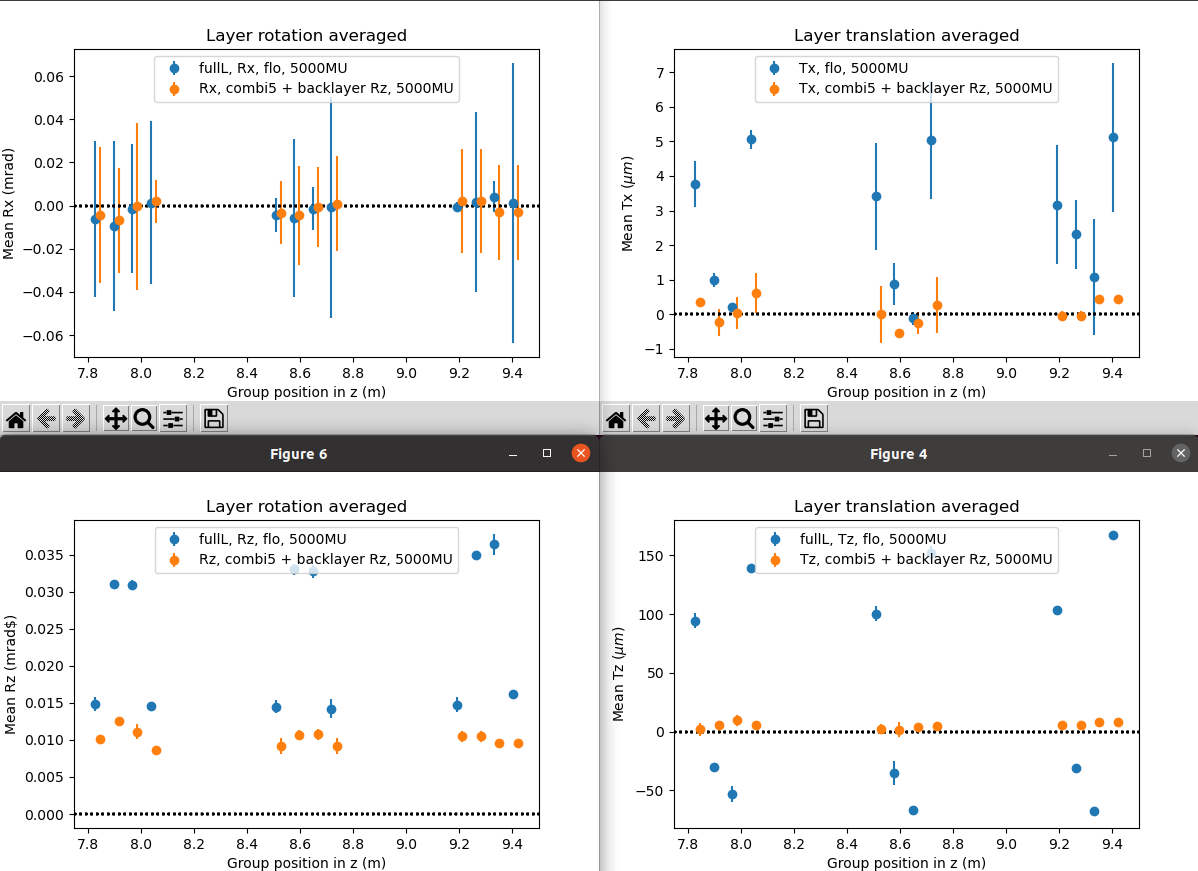
\includegraphics[width=0.8\textwidth]{plots/oct_6/combi5_added_RZ_backlayer.png}
  \caption{combi 5 with Rz backlayer constraint.}
  \label{fig:oct6}
\end{figure}

% november plots
\section{$\chi^2$ tests and weak modes}
In this section, $\chi^2$ are performed in order to study the "goodness" of the alignment since the better the $\chi^2$ after the alignment the better.
The second aspect i want to cover is the impact of potential weak modes also known as "correlated alignment parameters". There are several weak modes that could occur namely \textit{global translation}, \textit{shearing} and \textit{curvature bias}.
weak modes are unaffected by the $\chi^2$ since the residuals do not change.
The effect weak modes have on the alignment are biases regarding track parameters and late convergences.
There are different solutions that can be utilized to reduce the effect from weakmodes such as
\begin{itemize}
  \item \symbf{using other configurations like magnet off or mass plots for off-axis events}
  \item \symbf{utilizing other survey data sets}
  \item \symbf{using kinematic and vertex constraints}
\end{itemize}\,.

\begin{figure}
  \centering
  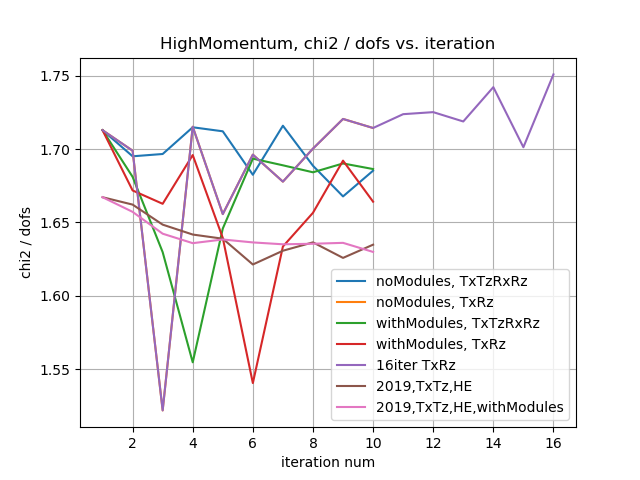
\includegraphics[width=0.8\textwidth]{plots/nov_19/Figure_2.png}
  \caption{chi2 vs iteration count.}
  \label{fig:fig2}
\end{figure}

\begin{figure}
  \centering
  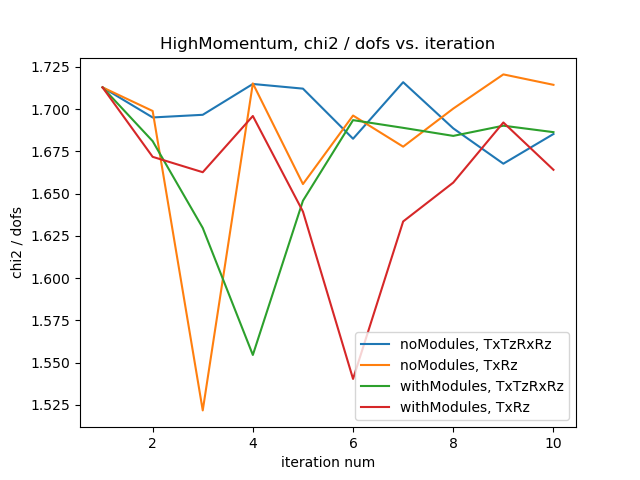
\includegraphics[width=0.8\textwidth]{plots/nov_21/chi2_vs_iter_all.png}
  \caption{chi2 versus iteration count.}
  \label{fig:chi2iter}
\end{figure}

\begin{figure}
  \centering
  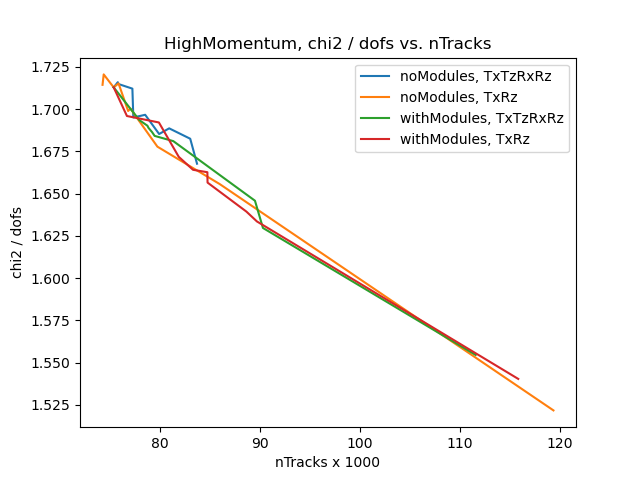
\includegraphics[width=0.8\textwidth]{plots/nov_21/chi2_vs_ntracks_all.png}
  \caption{chi2 versus number of tracks.}
  \label{fig:chi2tracks}
\end{figure}

% december plots
\begin{figure}
  \centering
  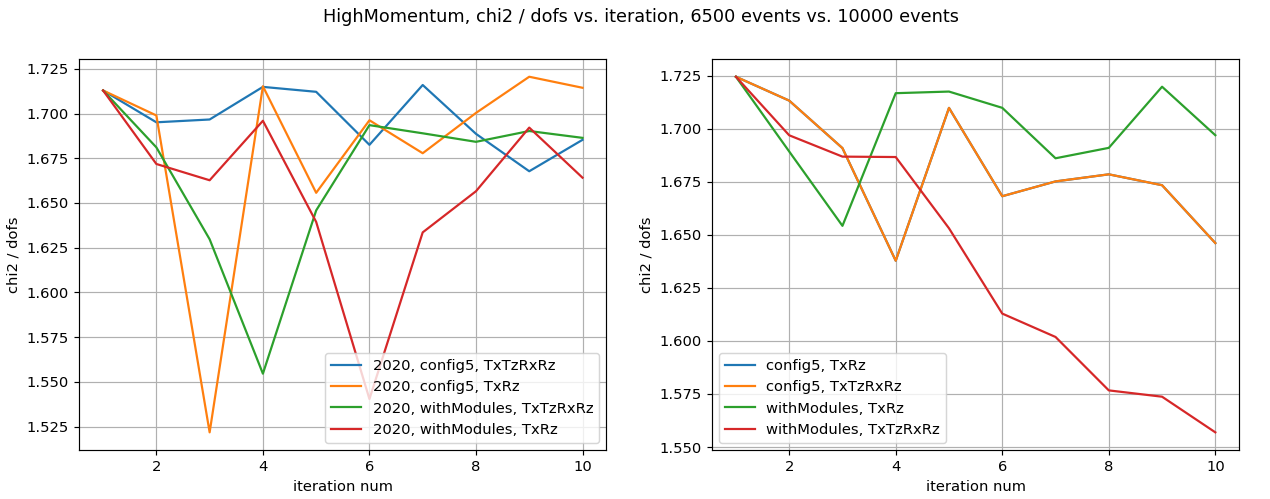
\includegraphics[width=0.8\textwidth]{plots/LHCB_week_dec/chi2_vs_iter_normal.png}
  \caption{chi2 versus iteration count normal(?).}
  \label{fig:chi2iterdec}
\end{figure}

\begin{figure}
  \centering
  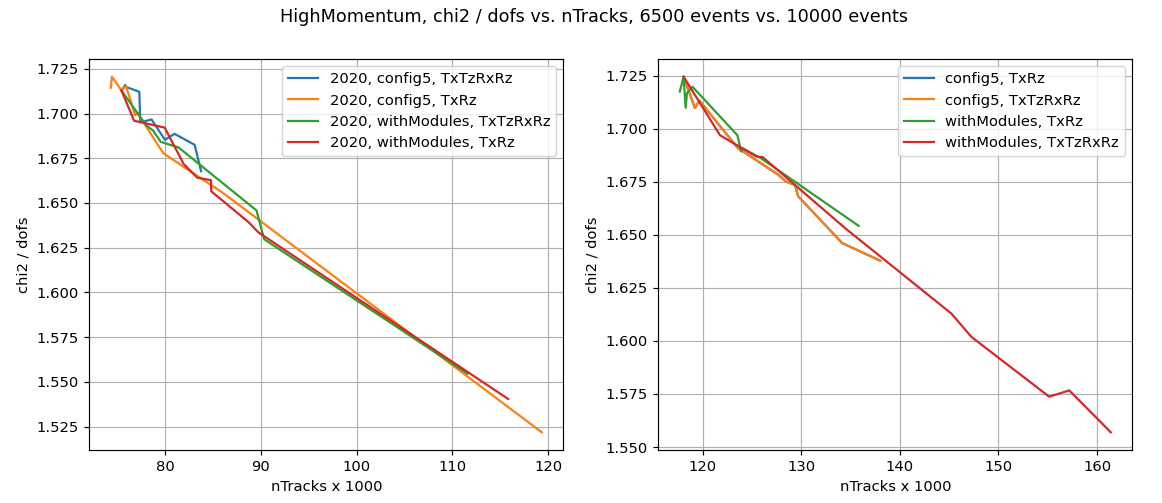
\includegraphics[width=0.8\textwidth]{plots/LHCB_week_dec/chi2_vs_tracks_normal.png}
  \caption{chi2 versus number of tracks normal.}
  \label{fig:chi2tracksdec}
\end{figure}

% january plats
january 17th plots are for luminosity comparisons.
nu for ramp up luminosity versus lumi during data taking.

\begin{figure}
  \centering
  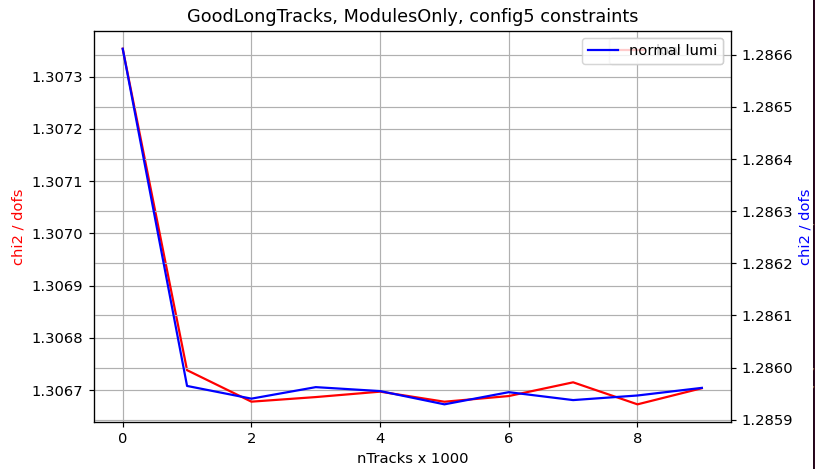
\includegraphics[width=0.8\textwidth]{plots/jan_17_2022/chi2_iter_low_vs_normal.png}
  \caption{compare different luminosities and plot chi2 versus iteration number as a measurement for weakmodes and alignment.}
  \label{fig:chi2iter_lumi_normal}
\end{figure}

for figure \ref{fig:chi2iter_lumi_normal} redo the plot with correct labels!!

\begin{figure}
  \centering
  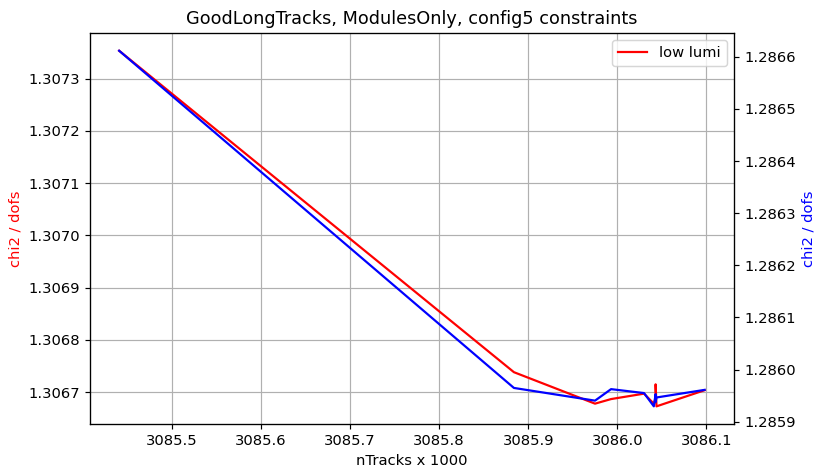
\includegraphics[width=0.8\textwidth]{plots/jan_17_2022/chi2_tracks_modulesOnly.png}
  \caption{compare different luminosities and plot chi2 versus number of tracks as a measurement for weakmodes and alignment.}
  \label{fig:chi2tracks_lumi_normal}
\end{figure}

\begin{figure}
  \centering
  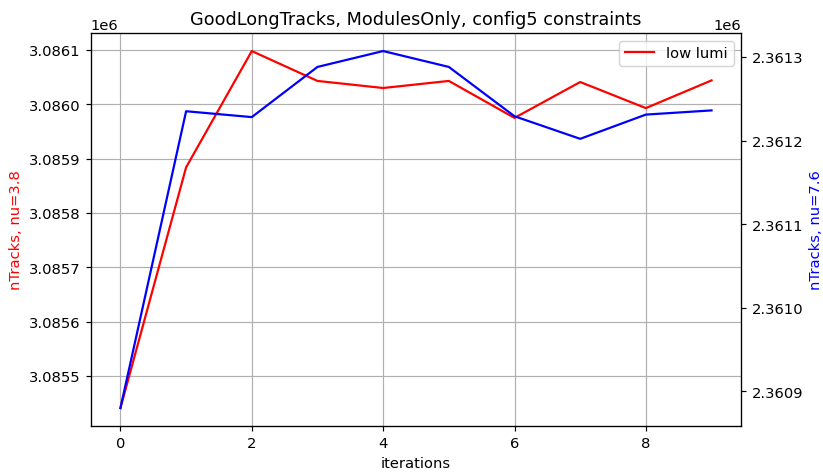
\includegraphics[width=0.8\textwidth]{plots/jan_17_2022/tracks_vs_iterations_modulesOnly.png}
  \caption{compare different luminosities and plot number of tracks versus iteration number as a measurement for weakmodes and alignment.}
  \label{fig:chi2iter_lumi_normal}
\end{figure}

january 24th: show that there is a visible difference between low and normal luminosity however the difference is not big enough to differentiate between the two phases during the ramp up and full run. therefore, for the upcoming analysis steps only the "normal/low" luminosity is taken into consideration.

\begin{figure}
  \centering
  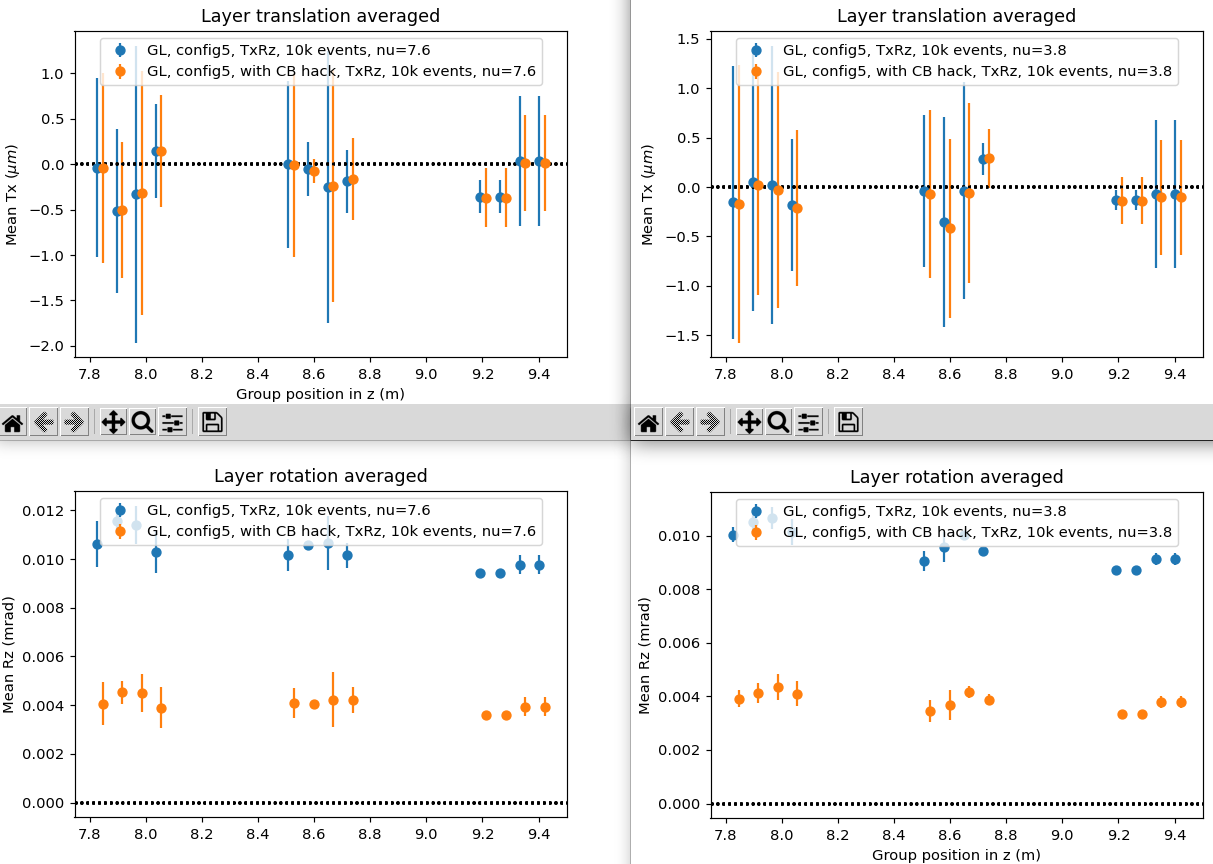
\includegraphics[width=0.8\textwidth]{plots/jan_24_2022/compare_with_without_hack.png}
  \caption{because of the clusterbias hack the difference between a measurement with the hack we implemented active and without is shown.}
  \label{fig:cbhack_on_off}
\end{figure}

\begin{figure}
  \centering
  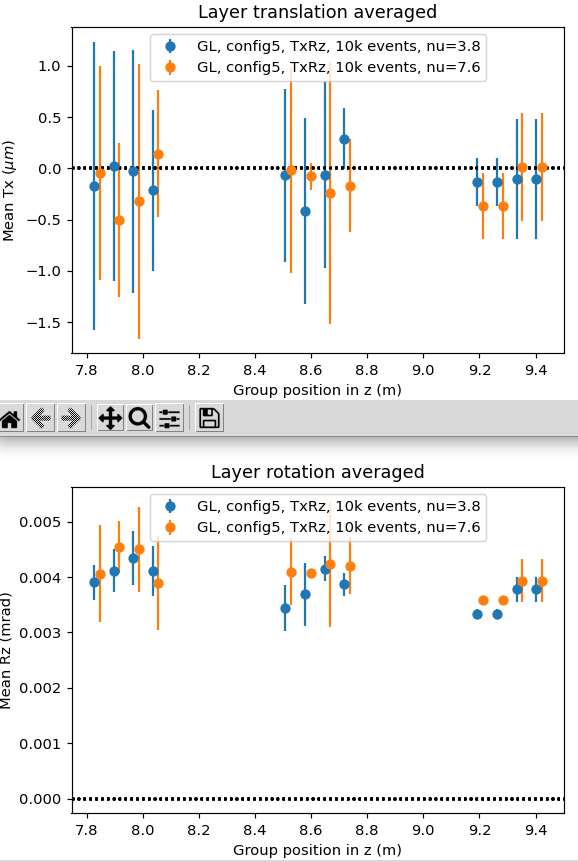
\includegraphics[width=0.8\textwidth]{plots/jan_24_2022/low_normal_with_hack.png}
  \caption{show difference between low and normal luminosity with clusterbias hack active.}
  \label{fig:lumi_low_normal_hack_on}
\end{figure}

% february plots
\begin{figure}
  \centering
  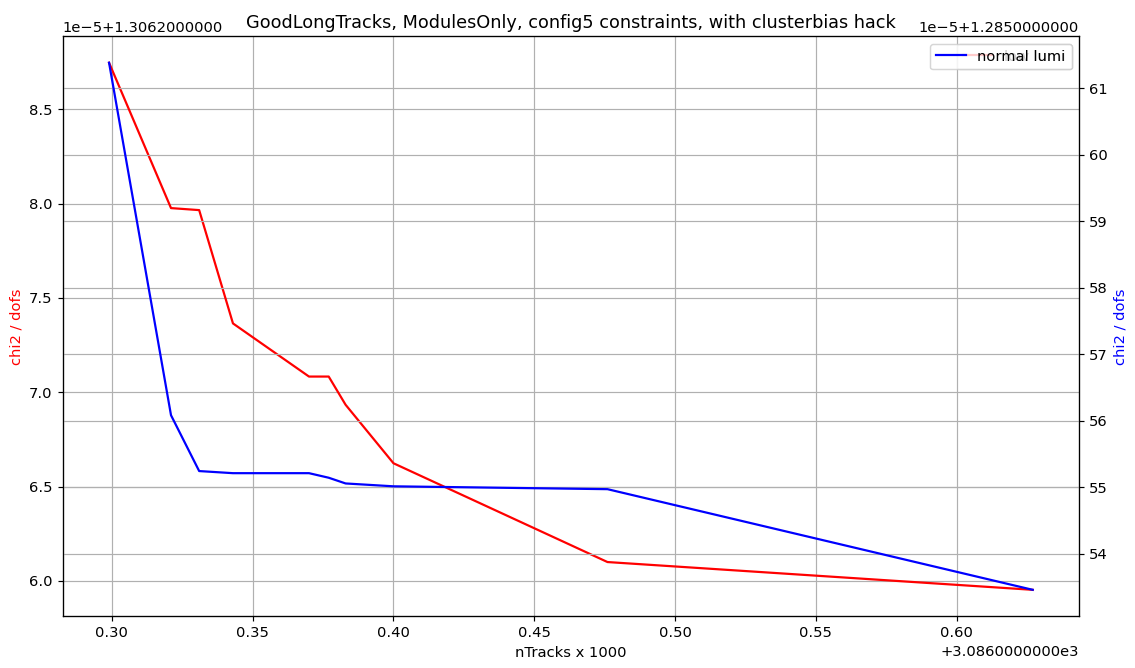
\includegraphics[width=0.8\textwidth]{plots/feb_2_2022/GL_modules_c5_cb_hackactive_low_normal_lumi.png}
  \caption{GoodLong tracks for module alignment and config 5 active. also the clusterbias hack is active comparing low and normal luminosity.}
  \label{fig:GL_lumi_low_normal_hack_on}
\end{figure}

\begin{figure}
  \centering
  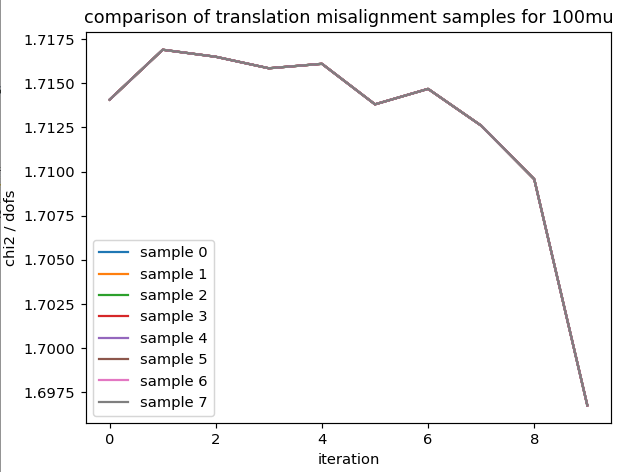
\includegraphics[width=0.8\textwidth]{plots/feb_6_2022/100mu_misalignment_samples_compared.png}
  \caption{100mu translation misalignment comparison for different misalignment samples.}
  \label{fig:100muT}
\end{figure}

\begin{figure}
  \centering
  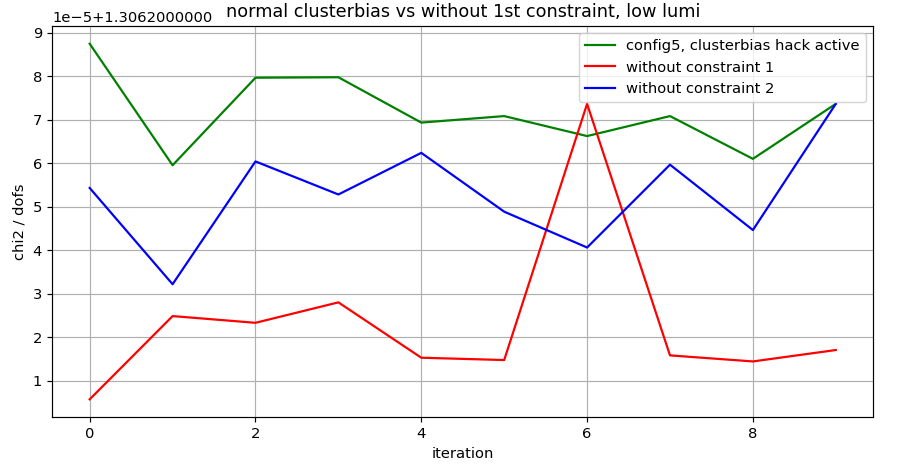
\includegraphics[width=0.8\textwidth]{plots/feb_6_2022/low_lumi_removed_constraints_vs_normal.png}
  \caption{impact of removing constraints from exisiting studies regarding chi2.}
  \label{fig:removeConst}
\end{figure}

% plan on how to sort things
% sources from me:   1. little notebook for first part
% after it was full: 2. sheets with dates
